\begin{figure}[ht]
	\begin{subfigure}[b]{0.32\linewidth}
		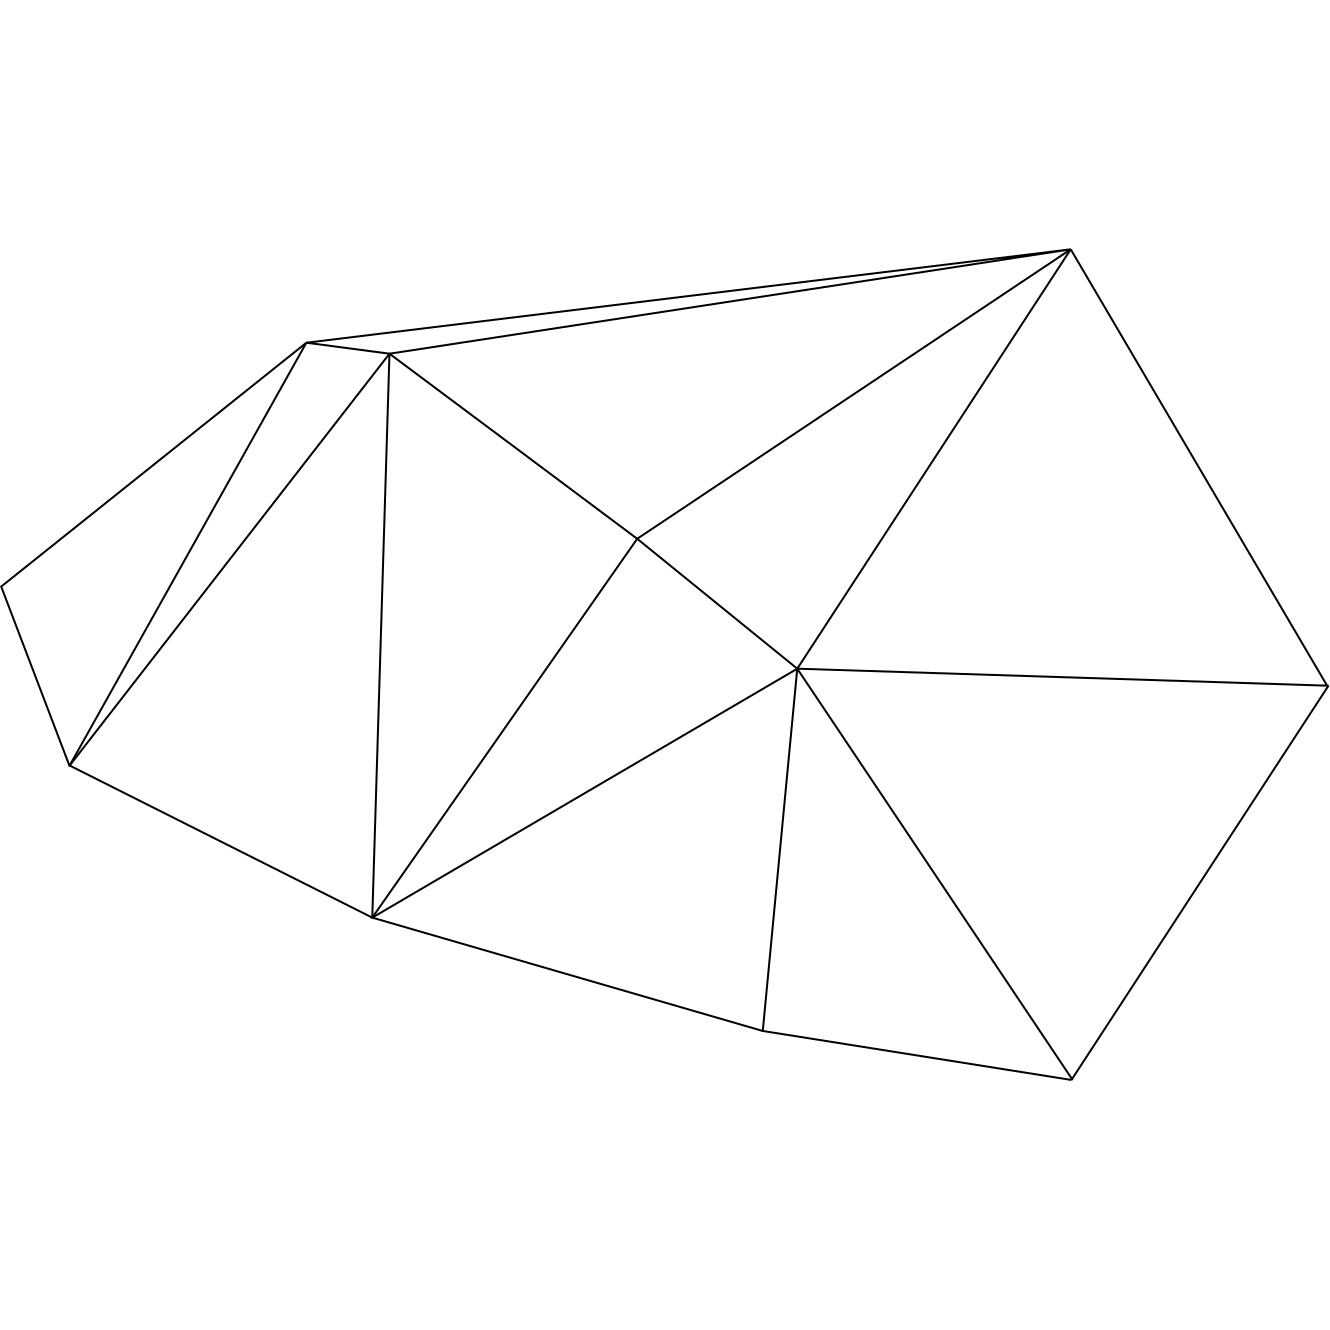
\includegraphics[width=\linewidth]
		{data/synthetic_meshes/random_circle_tessellation_Dirac_delta_1_v11_f12_wireframe.png}
		\caption{R=10, P=11, wireframe}\label{fig:rcirc.a}
	\end{subfigure}
	\begin{subfigure}[b]{0.32\linewidth}
		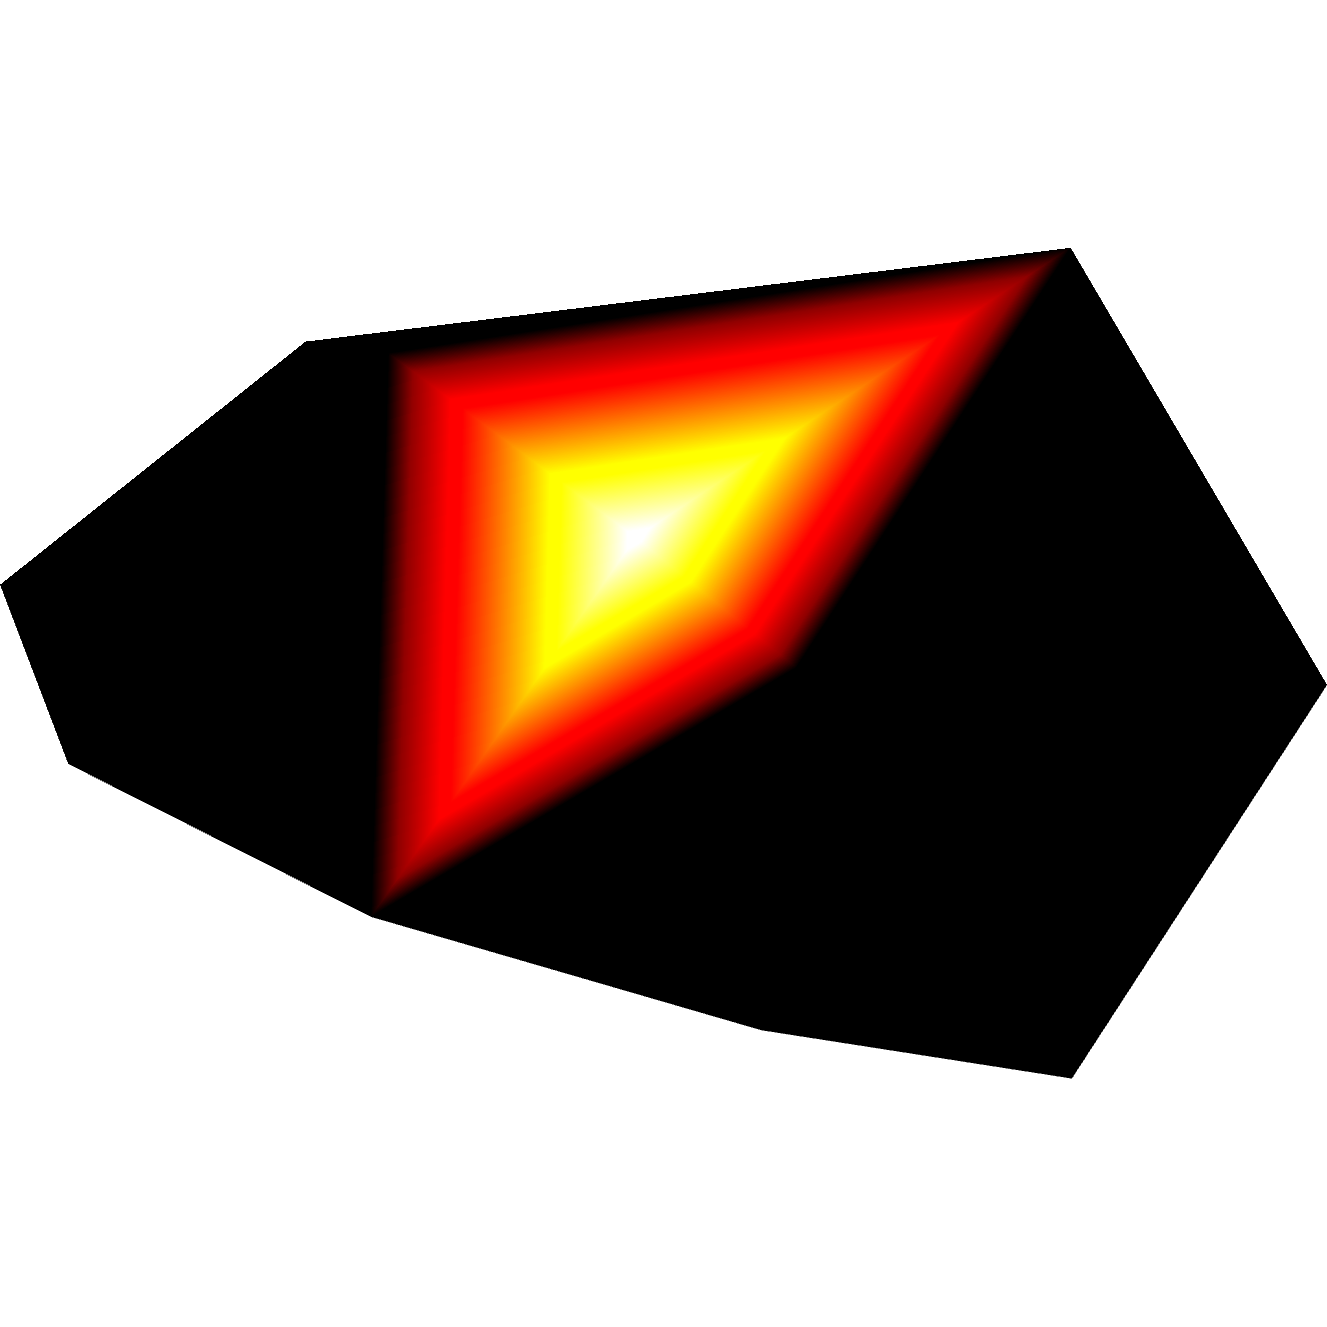
\includegraphics[width=\linewidth]
		{data/synthetic_meshes/random_circle_tessellation_Dirac_delta_1_v11_f12_funcvals_0iter.png}
		\caption{R=10, P=11, convolutions 0}\label{fig:rcirc.c}
	\end{subfigure}
	\begin{subfigure}[b]{0.32\linewidth}
		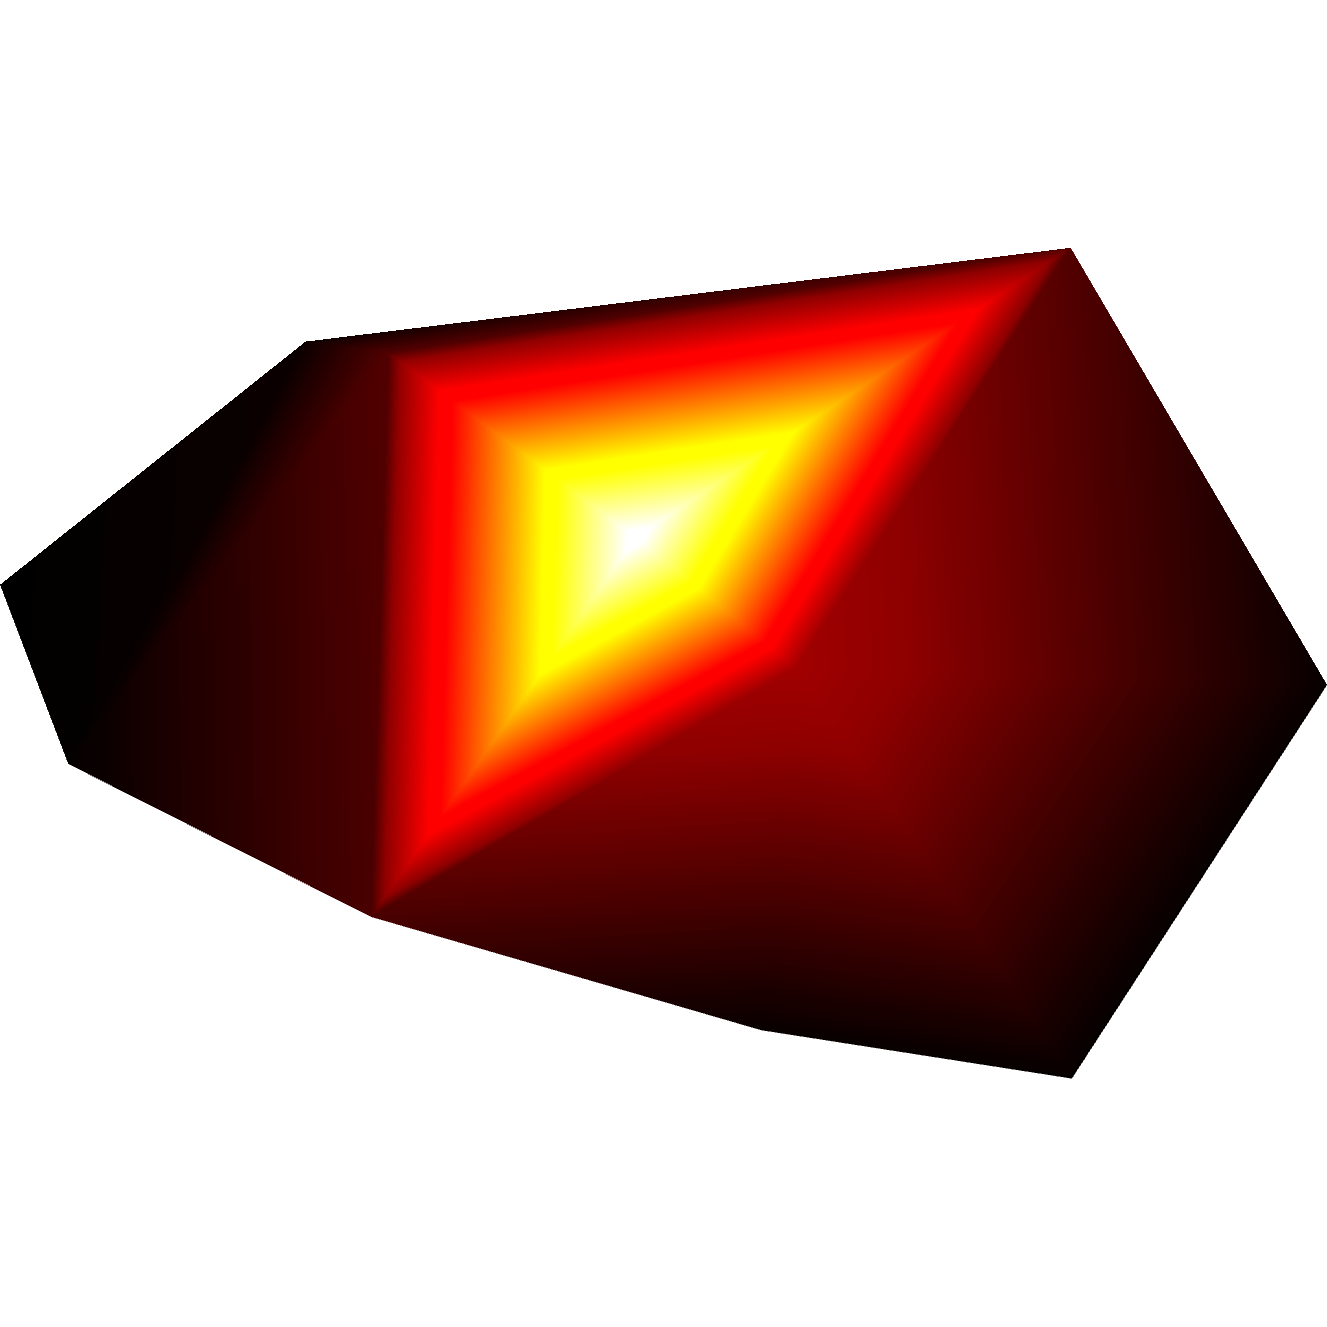
\includegraphics[width=\linewidth,]
		{data/synthetic_meshes/random_circle_tessellation_Dirac_delta_1_v11_f12_funcvals_2iter.png}
		\caption{R=10, P=11, convolutions 2}\label{fig:rcirc.e}
	\end{subfigure}

	\bigskip
	\begin{subfigure}[b]{0.32\linewidth}
		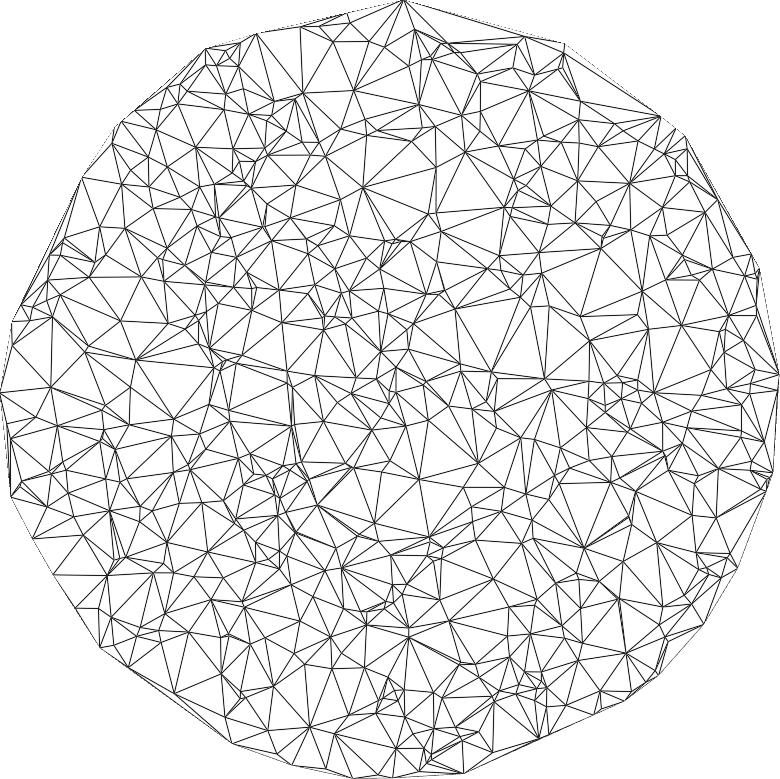
\includegraphics[width=\linewidth]
		{data/synthetic_meshes/random_circle_tessellation_Dirac_delta_10_v641_f1252_wireframe.png}
		\caption{R=10, P=641, convolutions}\label{fig:rcirc.b}
	\end{subfigure}
	\begin{subfigure}[b]{0.32\linewidth}
		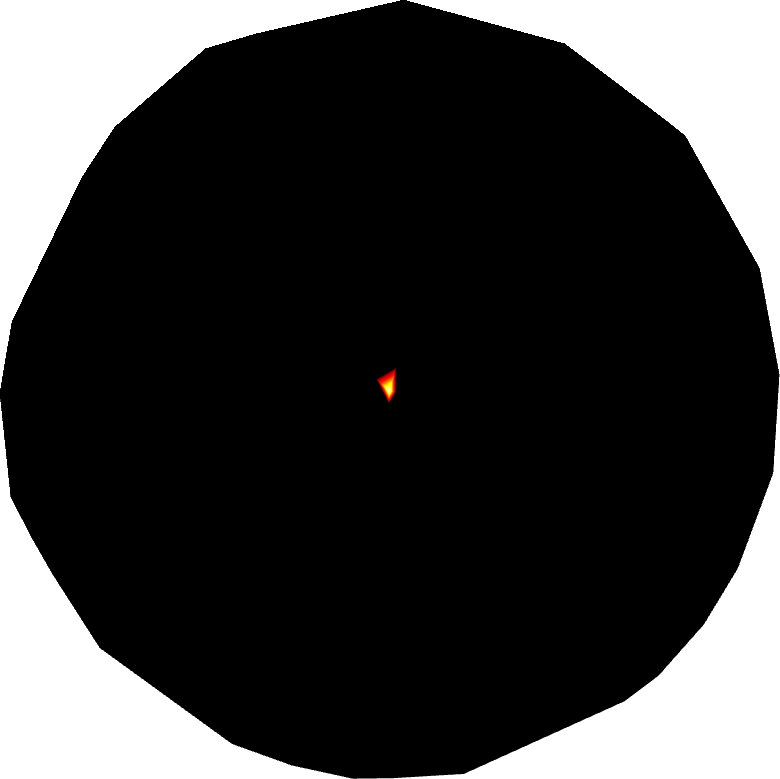
\includegraphics[width=\linewidth]
		{data/synthetic_meshes/random_circle_tessellation_Dirac_delta_10_v641_f1252_funcvals_0iter.png}
		\caption{R=10, P=641, convolutions 0}\label{fig:rcirc.d}
	\end{subfigure}
	\begin{subfigure}[b]{0.32\linewidth}
		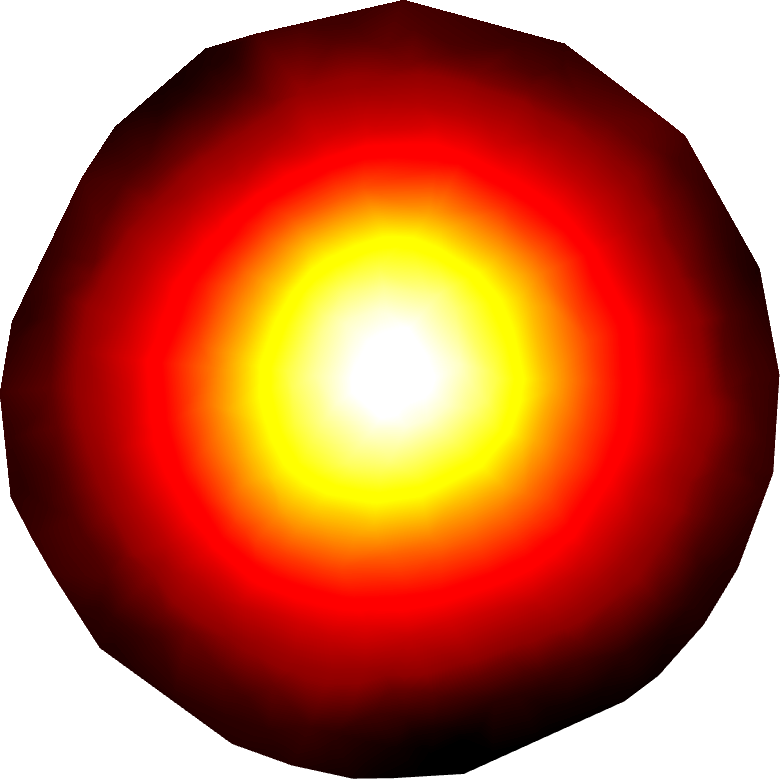
\includegraphics[width=\linewidth]
		{data/synthetic_meshes/random_circle_tessellation_Dirac_delta_10_v641_f1252_funcvals_10000iter.png}
		\caption{R=10, P=641, convolutions 10,000}\label{fig:rcirc.f}
	\end{subfigure}
	\caption[Six views, comparing two differently sized, random triangulated discs]{Comparison of two differently sized, random triangulated discs, generated with parameters R set to 1 and 10, and parameters P set to 11 and 641: (a) R=1, P=11 in wireframe (b) R=1, P=11 colored by function value before convolving the filter (c) R=1, P=11 colored by function value after convolving the filter twice (d) R=10, P=641 in wireframe (e) R=10, P=641 colored by function value before convoving the filter (f) R=10, P=641 colored by function value after convolving the filter 10,000 times.}
	\label{fig:rdisc}
\end{figure}

